% --------------------------------------------------------------------------- %
% Poster for the ECCS 2011 Conference about Elementary Dynamic Networks.      %
% --------------------------------------------------------------------------- %
% Created with Brian Amberg's LaTeX Poster Template. Please refer for the     %
% attached README.md file for the details how to compile with `pdflatex`.     %
% --------------------------------------------------------------------------- %
% $LastChangedDate:: 2011-09-11 10:57:12 +0200 (V, 11 szept. 2011)          $ %
% $LastChangedRevision:: 128                                                $ %
% $LastChangedBy:: rlegendi                                                 $ %
% $Id:: poster.tex 128 2011-09-11 08:57:12Z rlegendi                        $ %
% --------------------------------------------------------------------------- %
% Amended by Lev Landau------------------------------------------------------ %
% Amended by Preet Singh July 2013------------------------------------------- %

%\documentclass[paperwidth=42in,paperheight=56in,portrait]{baposter}
\documentclass[a0paper,portrait]{baposter}
\usepackage{amsmath}
\usepackage{amssymb}
\usepackage{relsize}	
\usepackage[numbers]{natbib}
	% For \smaller
\usepackage{url}			% For \url
\usepackage{epstopdf}	% Included EPS files automatically converted to PDF to include with pdflatex
\usepackage{caption}
%\usepackage{axodraw}
\usepackage{subfigure}

%%% Global Settings %%%%%%%%%%%%%%%%%%%%%%%%%%%%%%%%%%%%%%%%%%%%%%%%%%%%%%%%%%%
\renewcommand{\bibfont}{\footnotesize}
\graphicspath{{plots/}}	% Root directory of the pictures 
\tracingstats=2			% Enabled LaTeX logging with conditionals

%%% Color Definitions %%%%%%%%%%%%%%%%%%%%%%%%%%%%%%%%%%%%%%%%%%%%%%%%%%%%%%%%%

\definecolor{bordercol}{RGB}{40,40,40}
\definecolor{headercol1}{RGB}{186,215,230}
\definecolor{headercol2}{RGB}{80,80,80}
\definecolor{headerfontcol}{RGB}{0,0,0}
%\definecolor{boxcolor}{RGB}{186,215,230}
\definecolor{boxcolor}{RGB}{255,255,255}


%%%%%%%%%%%%%%%%%%%%%%%%%%%%%%%%%%%%%%%%%%%%%%%%%%%%%%%%%%%%%%%%%%%%%%%%%%%%%%%%
%%% Utility functions %%%%%%%%%%%%%%%%%%%%%%%%%%%%%%%%%%%%%%%%%%%%%%%%%%%%%%%%%%

%%% Save space in lists. Use this after the opening of the list %%%%%%%%%%%%%%%%
\newcommand{\compresslist}{
	\setlength{\itemsep}{1pt}
	\setlength{\parskip}{0pt}
	\setlength{\parsep}{0pt}
}

%%%%%%%%%%%%%%%%%%%%%%%%%%%%%%%%%%%%%%%%%%%%%%%%%%%%%%%%%%%%%%%%%%%%%%%%%%%%%%%
%%% Document Start %%%%%%%%%%%%%%%%%%%%%%%%%%%%%%%%%%%%%%%%%%%%%%%%%%%%%%%%%%%%
%%%%%%%%%%%%%%%%%%%%%%%%%%%%%%%%%%%%%%%%%%%%%%%%%%%%%%%%%%%%%%%%%%%%%%%%%%%%%%%

\begin{document}
\typeout{Poster rendering started}

%%% Setting Background Image %%%%%%%%%%%%%%%%%%%%%%%%%%%%%%%%%%%%%%%%%%%%%%%%%%
%\background{
%	\begin{tikzpicture}[remember picture,overlay]%
%	\draw (current page.north west)+(-2em,2em) node[anchor=north west]
%	{\includegraphics[height=1.1\textheight]{background}};
%	\end{tikzpicture}
%}

%%% General Poster Settings %%%%%%%%%%%%%%%%%%%%%%%%%%%%%%%%%%%%%%%%%%%%%%%%%%%
%%%%%% Eye Catcher, Title, Authors and University Images %%%%%%%%%%%%%%%%%%%%%%
\begin{poster}{
	grid=false,
	% Option is left on true though the eyecatcher is not used. The reason is
	% that we have a bit nicer looking title and author formatting in the headercol
	% this way
	%eyecatcher=false, 
	borderColor=bordercol,
	headerColorOne=headercol1,
	headerColorTwo=headercol2,
	headerFontColor=headerfontcol,
	% Only simple background color used, no shading, so boxColorTwo isn't necessary
	boxColorOne=boxcolor,
	headershape=roundedright,
	headerfont=\Large\sf\bf,
	textborder=rectangle,
	background=none,
	headerborder=open,
  boxshade=plain,
	columns=3
}
%%% Eye Cacther %%%%%%%%%%%%%%%%%%%%%%%%%%%%%%%%%%%%%%%%%%%%%%%%%%%%%%%%%%%%%%%
{
	Eye Catcher, empty if option eyecatcher=false - unused
}
%%% Title %%%%%%%%%%%%%%%%%%%%%%%%%%%%%%%%%%%%%%%%%%%%%%%%%%%%%%%%%%%%%%%%%%%%%
{\sf\bf
	Control Complexity of Schulze Voting
}
%%% Authors %%%%%%%%%%%%%%%%%%%%%%%%%%%%%%%%%%%%%%%%%%%%%%%%%%%%%%%%%%%%%%%%%%%
{
	 Curtis Menton$^{1}$, Preetjot Singh$^{2}$\\
	 \scriptsize
	 $^1${Computer Science, University of Rochester, Rochester, NY, USA}
        \par
        $^2${EECS, Northwestern University, Evanston, IL, USA }
%	Computer Science,\hspace{2cm} EECS Dept, \\
%	University of Rochester\hspace{2cm} Northwestern University
	%{\smaller shashank@northwestern.edu}
}
%%% Logo %%%%%%%%%%%%%%%%%%%%%%%%%%%%%%%%%%%%%%%%%%%%%%%%%%%%%%%%%%%%%%%%%%%%%%
{
% The logos are compressed a bit into a simple box to make them smaller on the result
% (Wasn't able to find any bigger of them.)
\setlength\fboxsep{0pt}
\setlength\fboxrule{0pt}
	\fbox{
		\begin{minipage}{4cm}
			%\includegraphics[width=4em,height=4em]{urlogo}
			
\includegraphics[width=4.25cm]{combinedlogo.eps}
			 \\
%			\includegraphics[width=10em,height=4em]{dynanets_logo}
%			\includegraphics[width=4em,height=4em]{aitia_logo}
		\end{minipage}
	}
}

\headerbox{Overview}{name=intro,column=0,span=2, row=0}{
One critical area of Computational Social Choice is the study of voting rules that contain just the right amount of complexity - enough to discourage strategic behaviour, but not so much that calculating the winner is NP-hard. 
The Schulze voting rule, introduced recently by Marcus Schulze in 1997, has quickly gained a high degree of real-world use: Users include \textbf{Wikimedia}, the P\textbf{irate Party}, \textbf{MTV}, and \textbf{Ubuntu}, among others. It is a Condorcet voting rule with a complex winner determination method that is nevertheless in polynomial time. Our paper resolves the complexity of several electoral \textit{control} cases, demonstrating previously unknown vulnerabilities and resistances of the voting rule.


%\phantom{\small{xxx}}
}
\headerbox{Definitions}{name=intro2,column=2,row=0}{
An \emph{election} is a pair $(C,V)$ where $C$ is a set of candidates and $V$
is a collection of votes. \textit{Votes} are preferences over candidates, expressed (in our case) as a strict linear ordering (such as $A > B >  C$ indicating $A$ is preferred to $B$ is preferred to $C$). A \emph{voting rule} is a mapping from an election $(C,V)$ to a set
$C' \subseteq C$ of winners.  \phantom{\small{xxxxxxxxxxxxxxxxxxxxxxxxxxxxxxxxxxx}}

}
\headerbox{How Schulze Finds The Winner}{name=definitions,column=0, span=3, below=intro}{
%Winner-calculation is a two-step process: 
%\begin{itemize}
%
%\item Generate weighted digraph based on \textit{netadv} scores.
%\item Obtain a secondary graph based on \textit{best paths} between any pair of candidates.
%\item Source of secondary graph is the winner. 
%\end{itemize}
\phantom{\small{xxxxxxxxxxxxxxxxxxxxxxxxxxxxxxxxxxxxxxxxxxxxxxxxxxxx}} 
\begin{tabular}{c c c c c}
%\begin{center}
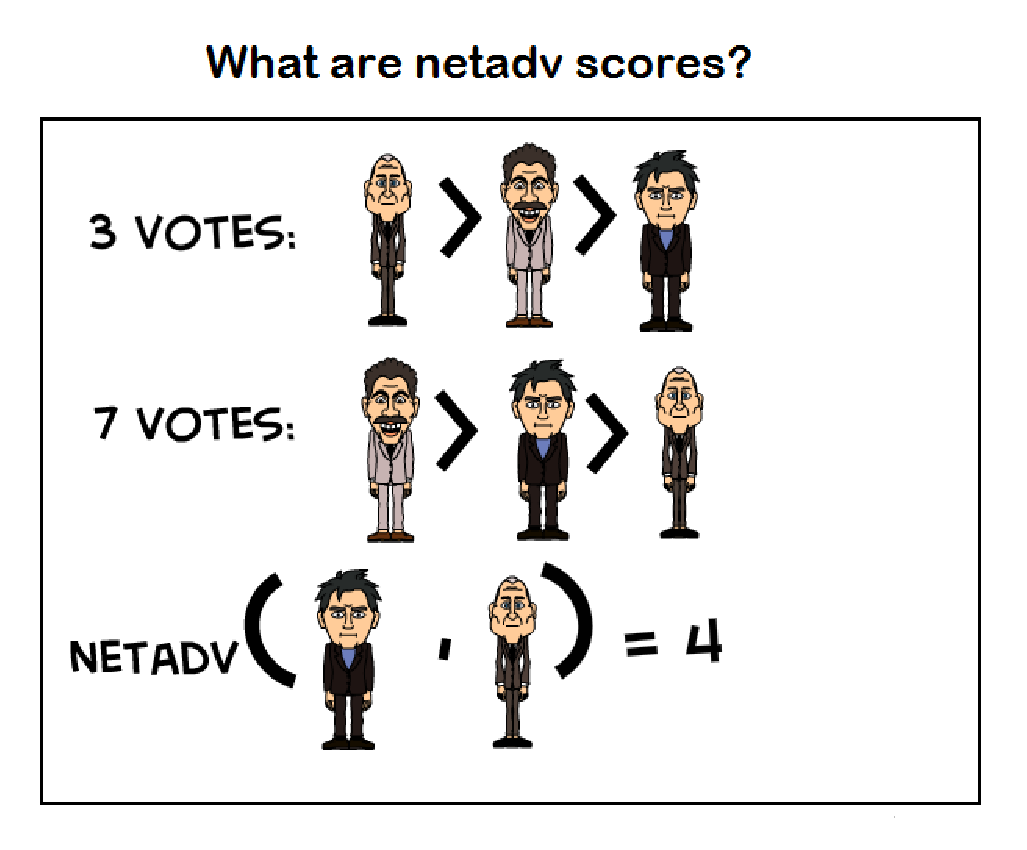
\includegraphics[width=0.18\linewidth]{netadv_expln.eps} &  
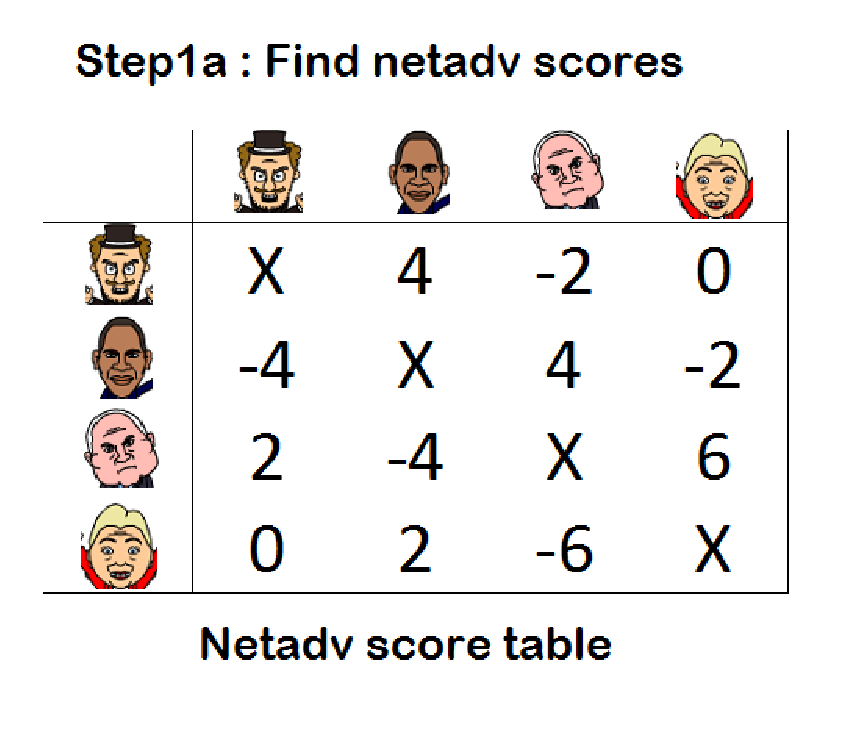
\includegraphics[width=0.18\linewidth]{netadv_scores_final.eps} & 
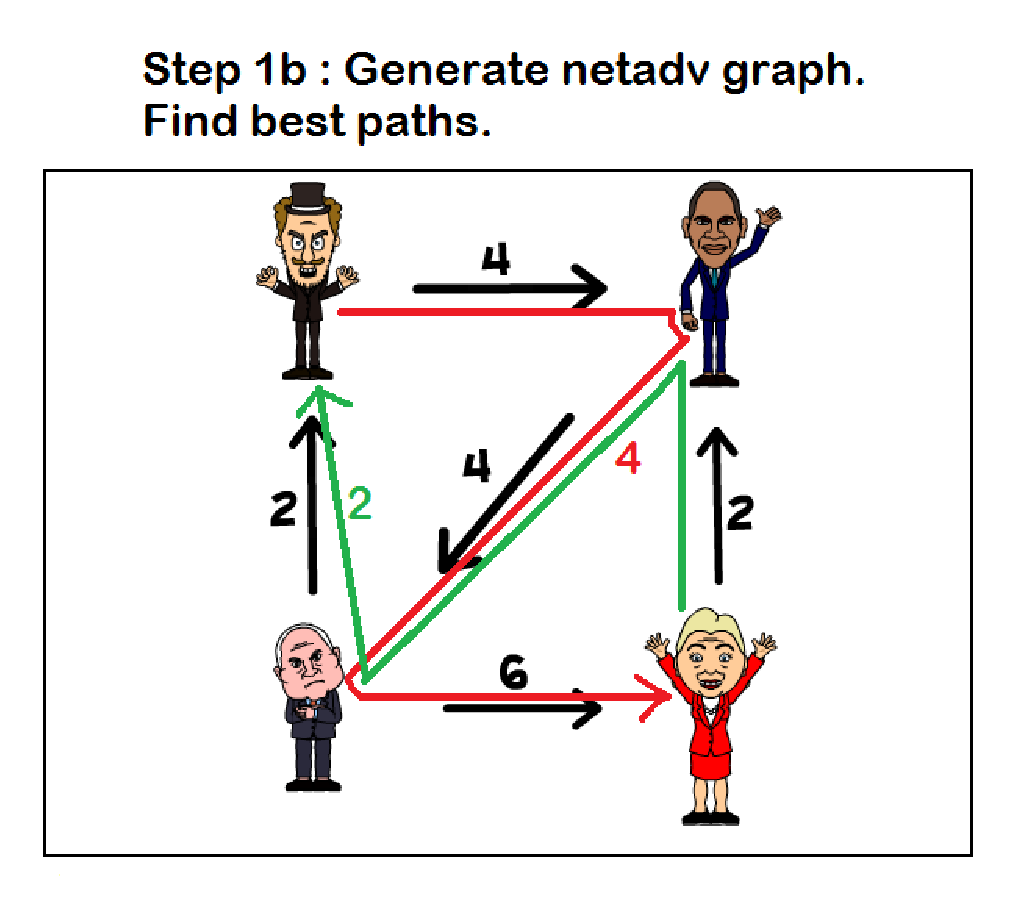
\includegraphics[width=0.18\linewidth]{netadv_graph.eps} &
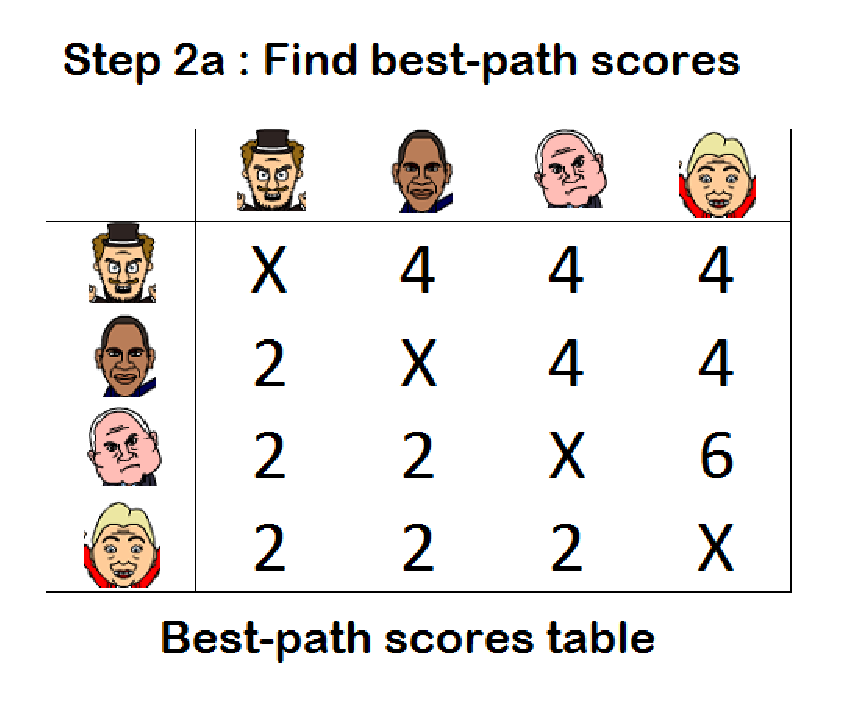
\includegraphics[width=0.18\linewidth]{Schulze_bestpath_scores.eps} & 
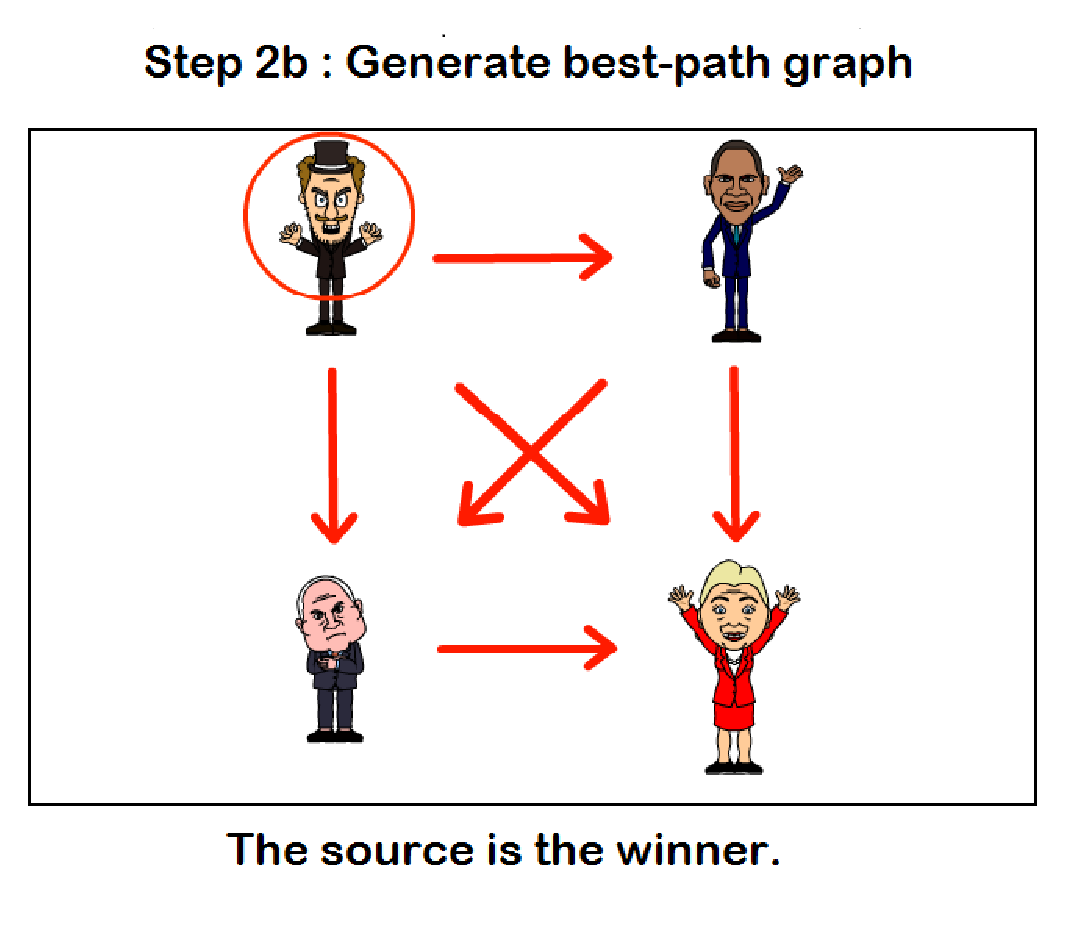
\includegraphics[width=0.18\linewidth]{Schulze_bestpathGraph.eps} 

%\end{center}
\end{tabular}

}

\headerbox{Control}{name=models,column=0, span=2, below=definitions}{
\textit{\textbf{Control}} refers to a class of manipulative actions that alter
the structure of an election to change the result. We model these as decision problems where we determine whether a case of control is possible in a given instance.

Control cases include:
\begin{itemize}
\itemsep0em
\item Adding or deleting voters (voter registration drives or voter suppression efforts).
\item Adding or deleting candidates (ballot-access procedures).
\item Partitioning voters (gerrymandering). 
\item Partitioning candidates (primary elections or runoff elections). 
\end{itemize}

}

\headerbox{Results}{name=magfield,column=0,span=2, below=models}
{
% TODO longer caption, explaining inclusions.
%\begin{table*}

  \centering

  \begin{tabular}{|l|l||l|l|l|l|l|l|l|l|}
    \hline
    Control by & Tie & 
    \multicolumn{2}{|c|}{Plurality} & \multicolumn{2}{|c|}{Approval} &  \multicolumn{2}{|c|}{Fallback} &
    \multicolumn{2}{|c|}{Schulze} \\
    & Model & C& D & C& D & C& D & C& D \\
    \hline \hline
    Adding Candidates & & R & R & I & V  & R & R & R & S\\
    \hline
    Adding Candidates (unlimited)  & & R & R & I & V & R & R & \textbf{R} & S \\
    \hline
    Deleting Candidates & & R & R & V & I & R & R & \textbf{R} & S\\
    \hline
    Partition of Candidates & TE & R & R & V & I  & R & R & \textbf{R} & \textbf{V}\\
    \hline
    & TP & R & R & I & I  & R & R & \textbf{R} & \textbf{V} \\
    \hline
    Run-off Partition of Candidates & TE & R & R & V & I  & R & R & \textbf{R}    & \textbf{V}\\
    \hline
    & TP & R & R & I & I  & R & R & \textbf{R} & \textbf{V}\\
    \hline
    Adding Voters & & V & V & R & V & R & V & R & R\\
    \hline
    Deleting Voters & & V & V & R & V & R & V & R & R\\
    \hline
    Partition of Voters & TE & V & V & R & V & R & R & \textbf{R} & \textbf{R}\\
    \hline
    & TP & R & R & R & V & R & R & \textbf{R} & \textbf{R} \\
    \hline
  \end{tabular}
  \captionof{figure}{Control behavior under Schulze voting and other voting
    systems for comparison.  V, R, S, and I stand for vulnerable, resistant,
    susceptible, and immune.  Results proved in this paper in bold,
    other results from~\protect\cite{erd-rot:c:fallback,erd-fel:c:param,erd-pir-rot:c:open-probs,hem-hem-rot:j:destructive-control,par-xia:c:ranked-pairs}.}
%  \caption{  \label{control-table}Control behavior under Schulze voting and other voting
%    systems for comparison.  V, R, S, and I stand for vulnerable, resistant,
%    susceptible, and immune.  Results proved in this paper in bold,
%    other results from~\protect\cite{erd-rot:c:fallback,erd-fel:c:param,erd-pir-%rot:c:open-probs,hem-hem-rot:j:destructive-control,par-xia:c:ranked-pairs}.}

%\end{table*}



%Due to the sudden collapse of the star, the magnetic flux is compressed in a small volume. The resulting magnetic field is extremely strong. In our simulation we use the following profile of the magnetic field.
%\begin{equation}
%B(r) = \left(\frac{50}{r (km)}\right)^{2} 10^{12} \ gauss \nonumber
%\end{equation}

%\phantom{\tiny{xx}}
}
\headerbox{References}{name=references,column=0,span=3, below=magfield}{
\renewcommand{\refname}{\vspace{-0.8em}}
          \bibliographystyle{abbrv}
          \bibliography{grycurtis}

%\smaller													% Make the whole text smaller
%\vspace{-0.4em} 										% Save some space at the beginning
%\bibliographystyle{plain}							% Use plain style
%\renewcommand{\section}[2]{\vskip 0.05em}		% Omit "References" title
%\begin{thebibliography}{1}							% Simple bibliography with widest label of 1
%\itemsep=-0.01em										% Save space between the separation
%\setlength{\baselineskip}{0.4em}					% Save space with longer lines
%\bibitem{deGouvea:2012hg} 
%  A.~de Gouvea and S.~Shalgar,
  %``Effect of Transition Magnetic Moments on Collective Supernova Neutrino Oscillations,''
%  JCAP {\bf 1210}, 027 (2012)
 % [arXiv:1207.0516 [astro-ph.HE]].
  %%CITATION = ARXIV:1207.0516;%%
  %1 citations counted in INSPIRE as of 12 Mar 2013
%\cite{deGouvea:2013zp}
%\bibitem{deGouvea:2013zp} 
%A.~de Gouvea and S.~Shalgar,
%JCAP (accepted)
%[arXiv:1301.5637 [astro-ph.HE]].
%\end{thebibliography}
}

%\headerbox{Acknowledgements}{name=acknowledgements,column=0,below=references, above=bottom}{
%\smaller						% Make the whole text smaller
%\vspace{-0.4em}			% Save some space at the beginning
%This research was partially supported by the Hungarian Government (KMOP-1.1.2-08/1-2008-0002 ) and the European Union's Seventh Framework Programme: DynaNets, FET-Open project no. FET-233847 (\url{http://www.dynanets.org}). The supports are gratefully acknowledged.
%} 

%\headerbox{Equations of motion}{name=density,span=2,column=1,row=0}{

%\includegraphics[angle=-90,width=0.98\linewidth]{PA_and_ER_Models_statisticalMeasures}
%}
%\headerbox{Equations of motion}{name=eom,span=1,column=1}
%{
%The density matrix of the neutrinos in the interior of a core-collapse supernova evolves %according to the following equation
%\begin{equation}
%i\dot{\rho}=[\rho,H]. \nonumber
%\label{eq:time}
%\end{equation}


%\headerbox{R-process nucleosynthesis}{name=implication,span=1,column=1,below=eom}{
%Core-collapse supernovae are the most probable sites of r-process nucleosynthesis. The rate of r-process nucleosynthesis is strongly dependent on the flux of neutrons near the r-process sites, which in turn is strongly dependent on the ratio of neutrinos to anti-neutrinos in the vicinity. The large lepton number violation induced by collective effects in the interior of supernovae may significantly alter our understanding of this phenomenon.

%\phantom{\tiny{xx}}
%}
%\headerbox{Results}
%{name=degreeDistribution,span=1,column=2}{
%\begin{center}
%	\includegraphics[width=0.49\linewidth]{initial}
%        \includegraphics[width=0.49\linewidth]{potential}
%Initial flux assumed in the simulation(left). Matter and self-interaction %potential(right).
%\end{center}
%\begin{center}
%	\includegraphics[width=0.49\linewidth]{stable}
%	\includegraphics[width=0.49\linewidth]{stablenormal}
%\end{center}
%Flux at 225 km for inverted(left) and normal(right) mass hierarchy without the effect of %transition magnetic moment. 
%\begin{center}
%	\includegraphics[width=0.49\linewidth]{nsimuem2nu}
%	\includegraphics[width=0.49\linewidth]{nsimuem2anu}
%\end{center}
%Neutrino(left) and anti-neutrino(right) fluxes at 225 km for inverted mass hierarchy with %transition magnetic moment of the order predicted by standard model.
%\begin{center}
%        \includegraphics[width=0.49\linewidth]{nsimunormalem2nu}
%        \includegraphics[width=0.49\linewidth]{nsimunormalem2anu}
%\end{center}
%Neutrino(left) and anti-neutrino(right) fluxes at 225 km for normal mass hierarchy with transition magnetic moment of the order predicted by standard model.
%}
\headerbox{Control cases}{name=models1,column=2, above=references, below=definitions}{
\begin{tabular}{c}
%\begin{center}
\phantom{\tiny{xxxxx}}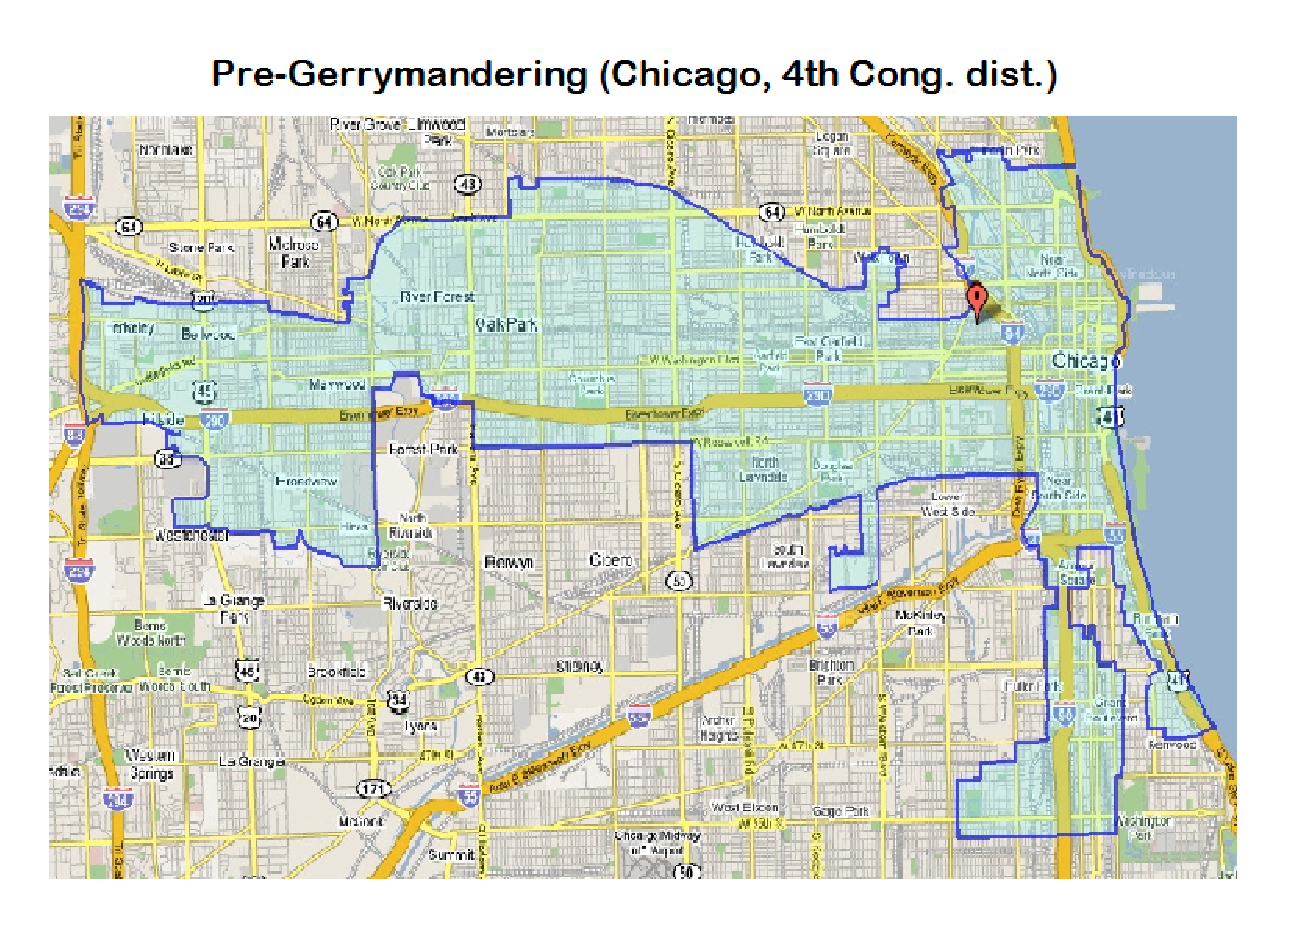
\includegraphics[width=0.75\linewidth]{pregerry.eps} \\
\phantom{\tiny{xxxxx}}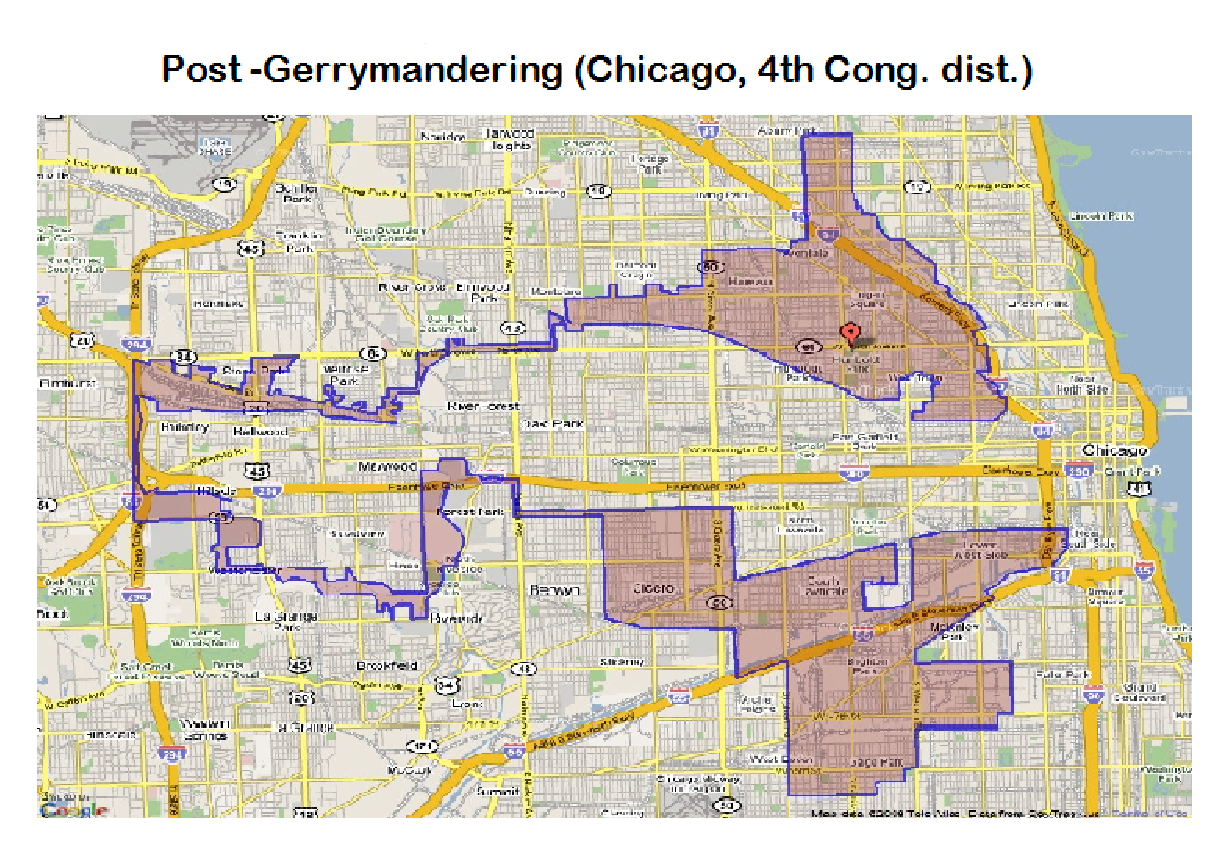
\includegraphics[width=0.75\linewidth]{postgerry.eps} \\
\phantom{\tiny{xxxxx}}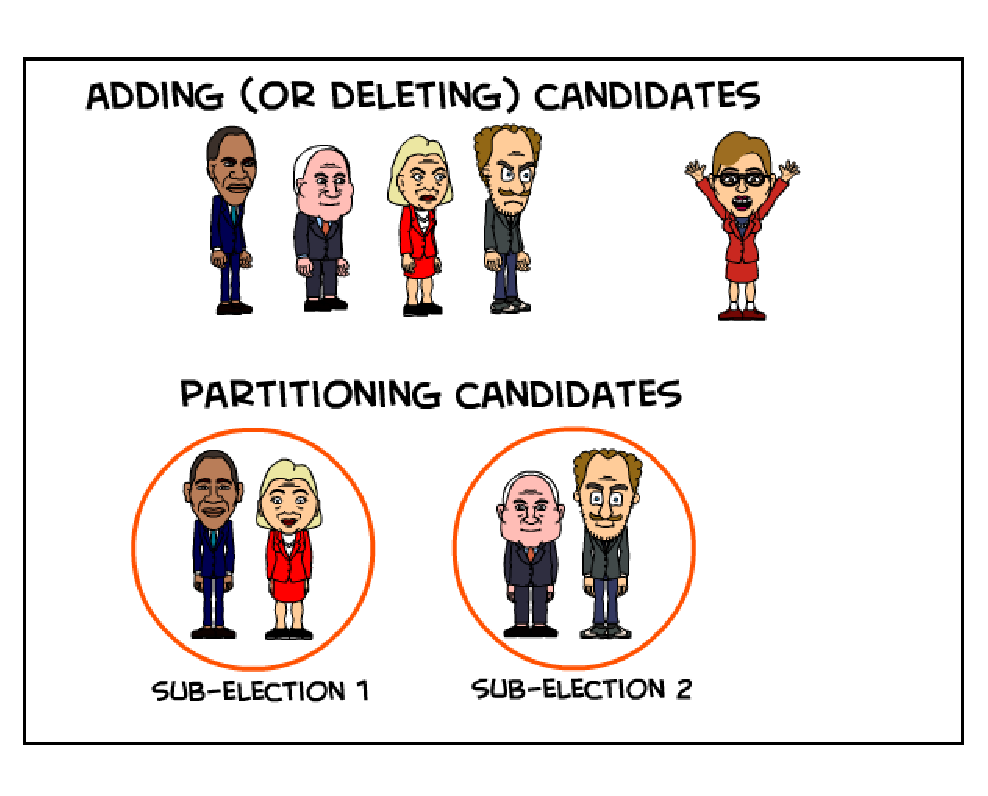
\includegraphics[width=0.75\linewidth]{addingcand.eps} 


%\end{center}
\end{tabular}
}
\end{poster}
\end{document}
